\documentclass[]{article}
\usepackage{lmodern}
\usepackage{amssymb,amsmath}
\usepackage{ifxetex,ifluatex}
\usepackage{fixltx2e} % provides \textsubscript
\ifnum 0\ifxetex 1\fi\ifluatex 1\fi=0 % if pdftex
  \usepackage[T1]{fontenc}
  \usepackage[utf8]{inputenc}
\else % if luatex or xelatex
  \ifxetex
    \usepackage{mathspec}
  \else
    \usepackage{fontspec}
  \fi
  \defaultfontfeatures{Ligatures=TeX,Scale=MatchLowercase}
\fi
% use upquote if available, for straight quotes in verbatim environments
\IfFileExists{upquote.sty}{\usepackage{upquote}}{}
% use microtype if available
\IfFileExists{microtype.sty}{%
\usepackage{microtype}
\UseMicrotypeSet[protrusion]{basicmath} % disable protrusion for tt fonts
}{}
\usepackage[margin=1in]{geometry}
\usepackage{hyperref}
\hypersetup{unicode=true,
            pdftitle={Workout 1 Report},
            pdfauthor={Elias Junior Ghantous},
            pdfborder={0 0 0},
            breaklinks=true}
\urlstyle{same}  % don't use monospace font for urls
\usepackage{color}
\usepackage{fancyvrb}
\newcommand{\VerbBar}{|}
\newcommand{\VERB}{\Verb[commandchars=\\\{\}]}
\DefineVerbatimEnvironment{Highlighting}{Verbatim}{commandchars=\\\{\}}
% Add ',fontsize=\small' for more characters per line
\usepackage{framed}
\definecolor{shadecolor}{RGB}{248,248,248}
\newenvironment{Shaded}{\begin{snugshade}}{\end{snugshade}}
\newcommand{\KeywordTok}[1]{\textcolor[rgb]{0.13,0.29,0.53}{\textbf{#1}}}
\newcommand{\DataTypeTok}[1]{\textcolor[rgb]{0.13,0.29,0.53}{#1}}
\newcommand{\DecValTok}[1]{\textcolor[rgb]{0.00,0.00,0.81}{#1}}
\newcommand{\BaseNTok}[1]{\textcolor[rgb]{0.00,0.00,0.81}{#1}}
\newcommand{\FloatTok}[1]{\textcolor[rgb]{0.00,0.00,0.81}{#1}}
\newcommand{\ConstantTok}[1]{\textcolor[rgb]{0.00,0.00,0.00}{#1}}
\newcommand{\CharTok}[1]{\textcolor[rgb]{0.31,0.60,0.02}{#1}}
\newcommand{\SpecialCharTok}[1]{\textcolor[rgb]{0.00,0.00,0.00}{#1}}
\newcommand{\StringTok}[1]{\textcolor[rgb]{0.31,0.60,0.02}{#1}}
\newcommand{\VerbatimStringTok}[1]{\textcolor[rgb]{0.31,0.60,0.02}{#1}}
\newcommand{\SpecialStringTok}[1]{\textcolor[rgb]{0.31,0.60,0.02}{#1}}
\newcommand{\ImportTok}[1]{#1}
\newcommand{\CommentTok}[1]{\textcolor[rgb]{0.56,0.35,0.01}{\textit{#1}}}
\newcommand{\DocumentationTok}[1]{\textcolor[rgb]{0.56,0.35,0.01}{\textbf{\textit{#1}}}}
\newcommand{\AnnotationTok}[1]{\textcolor[rgb]{0.56,0.35,0.01}{\textbf{\textit{#1}}}}
\newcommand{\CommentVarTok}[1]{\textcolor[rgb]{0.56,0.35,0.01}{\textbf{\textit{#1}}}}
\newcommand{\OtherTok}[1]{\textcolor[rgb]{0.56,0.35,0.01}{#1}}
\newcommand{\FunctionTok}[1]{\textcolor[rgb]{0.00,0.00,0.00}{#1}}
\newcommand{\VariableTok}[1]{\textcolor[rgb]{0.00,0.00,0.00}{#1}}
\newcommand{\ControlFlowTok}[1]{\textcolor[rgb]{0.13,0.29,0.53}{\textbf{#1}}}
\newcommand{\OperatorTok}[1]{\textcolor[rgb]{0.81,0.36,0.00}{\textbf{#1}}}
\newcommand{\BuiltInTok}[1]{#1}
\newcommand{\ExtensionTok}[1]{#1}
\newcommand{\PreprocessorTok}[1]{\textcolor[rgb]{0.56,0.35,0.01}{\textit{#1}}}
\newcommand{\AttributeTok}[1]{\textcolor[rgb]{0.77,0.63,0.00}{#1}}
\newcommand{\RegionMarkerTok}[1]{#1}
\newcommand{\InformationTok}[1]{\textcolor[rgb]{0.56,0.35,0.01}{\textbf{\textit{#1}}}}
\newcommand{\WarningTok}[1]{\textcolor[rgb]{0.56,0.35,0.01}{\textbf{\textit{#1}}}}
\newcommand{\AlertTok}[1]{\textcolor[rgb]{0.94,0.16,0.16}{#1}}
\newcommand{\ErrorTok}[1]{\textcolor[rgb]{0.64,0.00,0.00}{\textbf{#1}}}
\newcommand{\NormalTok}[1]{#1}
\usepackage{graphicx,grffile}
\makeatletter
\def\maxwidth{\ifdim\Gin@nat@width>\linewidth\linewidth\else\Gin@nat@width\fi}
\def\maxheight{\ifdim\Gin@nat@height>\textheight\textheight\else\Gin@nat@height\fi}
\makeatother
% Scale images if necessary, so that they will not overflow the page
% margins by default, and it is still possible to overwrite the defaults
% using explicit options in \includegraphics[width, height, ...]{}
\setkeys{Gin}{width=\maxwidth,height=\maxheight,keepaspectratio}
\IfFileExists{parskip.sty}{%
\usepackage{parskip}
}{% else
\setlength{\parindent}{0pt}
\setlength{\parskip}{6pt plus 2pt minus 1pt}
}
\setlength{\emergencystretch}{3em}  % prevent overfull lines
\providecommand{\tightlist}{%
  \setlength{\itemsep}{0pt}\setlength{\parskip}{0pt}}
\setcounter{secnumdepth}{0}
% Redefines (sub)paragraphs to behave more like sections
\ifx\paragraph\undefined\else
\let\oldparagraph\paragraph
\renewcommand{\paragraph}[1]{\oldparagraph{#1}\mbox{}}
\fi
\ifx\subparagraph\undefined\else
\let\oldsubparagraph\subparagraph
\renewcommand{\subparagraph}[1]{\oldsubparagraph{#1}\mbox{}}
\fi

%%% Use protect on footnotes to avoid problems with footnotes in titles
\let\rmarkdownfootnote\footnote%
\def\footnote{\protect\rmarkdownfootnote}

%%% Change title format to be more compact
\usepackage{titling}

% Create subtitle command for use in maketitle
\newcommand{\subtitle}[1]{
  \posttitle{
    \begin{center}\large#1\end{center}
    }
}

\setlength{\droptitle}{-2em}

  \title{Workout 1 Report}
    \pretitle{\vspace{\droptitle}\centering\huge}
  \posttitle{\par}
    \author{Elias Junior Ghantous}
    \preauthor{\centering\large\emph}
  \postauthor{\par}
      \predate{\centering\large\emph}
  \postdate{\par}
    \date{October 18, 2019}


\begin{document}
\maketitle

\begin{Shaded}
\begin{Highlighting}[]
\KeywordTok{library}\NormalTok{(readr)}
\end{Highlighting}
\end{Shaded}

\begin{verbatim}
## Warning: package 'readr' was built under R version 3.5.3
\end{verbatim}

\begin{Shaded}
\begin{Highlighting}[]
\KeywordTok{library}\NormalTok{(dplyr)}
\end{Highlighting}
\end{Shaded}

\begin{verbatim}
## Warning: package 'dplyr' was built under R version 3.5.3
\end{verbatim}

\begin{verbatim}
## 
## Attaching package: 'dplyr'
\end{verbatim}

\begin{verbatim}
## The following objects are masked from 'package:stats':
## 
##     filter, lag
\end{verbatim}

\begin{verbatim}
## The following objects are masked from 'package:base':
## 
##     intersect, setdiff, setequal, union
\end{verbatim}

\begin{Shaded}
\begin{Highlighting}[]
\KeywordTok{library}\NormalTok{(ggplot2)}
\end{Highlighting}
\end{Shaded}

\begin{verbatim}
## Warning: package 'ggplot2' was built under R version 3.5.3
\end{verbatim}

\begin{Shaded}
\begin{Highlighting}[]
\KeywordTok{library}\NormalTok{(lubridate)}
\end{Highlighting}
\end{Shaded}

\begin{verbatim}
## Warning: package 'lubridate' was built under R version 3.5.3
\end{verbatim}

\begin{verbatim}
## 
## Attaching package: 'lubridate'
\end{verbatim}

\begin{verbatim}
## The following object is masked from 'package:base':
## 
##     date
\end{verbatim}

What is the number of (unique) storms in each year? .What is the total
number of storms per hemisphere? .Do storms tend to occur more often in
one hemisphere than in the other? .Do storms tend to occur uniformly
throughout the year (evenly amount of storms permonth)? Or are there
months where there's more storm activity? .Is there a particular Basin
where storms occur more frequently? Or are there basinswithout much
storm activity? .What is the typical duration of a storm (e.g.~in terms
of hours, or days)? .Are there storms with durations that deviate
considerably from the typical duration? .What is the top-10 list of
storms in terms of high wind speed values?

\begin{Shaded}
\begin{Highlighting}[]
\NormalTok{dat <-}\StringTok{ }\KeywordTok{read_csv}\NormalTok{(}\StringTok{"../data/ibtracs-2010-2015.csv"}\NormalTok{, }\DataTypeTok{col_names =} \KeywordTok{c}\NormalTok{(}\StringTok{"serial_num"}\NormalTok{, }\StringTok{"season"}\NormalTok{, }\StringTok{"num"}\NormalTok{, }\StringTok{"basin"}\NormalTok{, }\StringTok{"sub_basin"}\NormalTok{, }\StringTok{"name"}\NormalTok{, }\StringTok{"iso_time"}\NormalTok{, }\StringTok{"nature"}\NormalTok{, }\StringTok{"latitude"}\NormalTok{, }\StringTok{"longitude"}\NormalTok{, }\StringTok{"wind"}\NormalTok{, }\StringTok{"press"}\NormalTok{), }\DataTypeTok{skip =} \DecValTok{1}\NormalTok{, }\DataTypeTok{col_types =} \KeywordTok{cols}\NormalTok{(}\KeywordTok{col_character}\NormalTok{(), }\KeywordTok{col_integer}\NormalTok{(), }\KeywordTok{col_character}\NormalTok{(), }\KeywordTok{col_factor}\NormalTok{(), }\KeywordTok{col_character}\NormalTok{(), }\KeywordTok{col_character}\NormalTok{(), }\KeywordTok{col_character}\NormalTok{(), }\KeywordTok{col_character}\NormalTok{(), }\KeywordTok{col_double}\NormalTok{(), }\KeywordTok{col_double}\NormalTok{(), }\KeywordTok{col_double}\NormalTok{(), }\KeywordTok{col_double}\NormalTok{()), }\DataTypeTok{na =} \KeywordTok{c}\NormalTok{(}\StringTok{"-999."}\NormalTok{, }\StringTok{"-1.0"}\NormalTok{, }\StringTok{"0.0"}\NormalTok{))}
\NormalTok{dat <-}\StringTok{ }\KeywordTok{as.data.frame}\NormalTok{(dat)}
\end{Highlighting}
\end{Shaded}

\begin{Shaded}
\begin{Highlighting}[]
\NormalTok{storms_per_year <-}\StringTok{ }\KeywordTok{count}\NormalTok{(}\KeywordTok{distinct}\NormalTok{(dat, season, name), season)}
\KeywordTok{ggplot}\NormalTok{(}\DataTypeTok{data =}\NormalTok{ storms_per_year, }\KeywordTok{aes}\NormalTok{(}\DataTypeTok{x =}\NormalTok{ season, }\DataTypeTok{y =}\NormalTok{ n)) }\OperatorTok{+}\StringTok{ }\KeywordTok{geom_bar}\NormalTok{(}\DataTypeTok{stat =} \StringTok{'identity'}\NormalTok{, }\DataTypeTok{fill =} \StringTok{"purple"}\NormalTok{) }\OperatorTok{+}\StringTok{ }\KeywordTok{geom_text}\NormalTok{(}\KeywordTok{aes}\NormalTok{(}\DataTypeTok{label =}\NormalTok{ n), }\DataTypeTok{vjust=}\OperatorTok{-}\FloatTok{0.5}\NormalTok{) }\OperatorTok{+}
\StringTok{  }\KeywordTok{xlab}\NormalTok{(}\StringTok{"Year"}\NormalTok{) }\OperatorTok{+}\StringTok{ }\KeywordTok{ylab}\NormalTok{(}\StringTok{"Count"}\NormalTok{) }\OperatorTok{+}\StringTok{ }\KeywordTok{ggtitle}\NormalTok{(}\StringTok{"Number of Unique Storms in Each Year"}\NormalTok{) }\OperatorTok{+}\StringTok{ }\KeywordTok{theme_minimal}\NormalTok{()}
\end{Highlighting}
\end{Shaded}

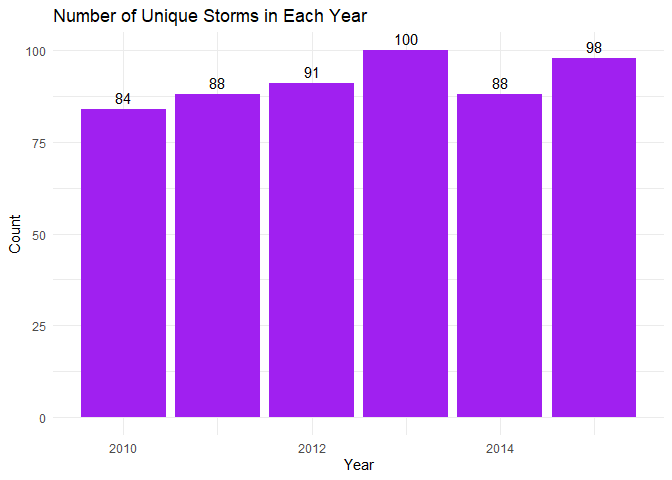
\includegraphics{workout1-elias-ghantous_files/figure-latex/unnamed-chunk-3-1.pdf}

\begin{Shaded}
\begin{Highlighting}[]
\CommentTok{#northern hemisphere}
\NormalTok{northhem =}\StringTok{ }\KeywordTok{count}\NormalTok{(}\KeywordTok{filter}\NormalTok{(dat, latitude }\OperatorTok{>=}\StringTok{ }\DecValTok{0}\NormalTok{), serial_num)}
\KeywordTok{nrow}\NormalTok{(northhem)}
\end{Highlighting}
\end{Shaded}

\begin{verbatim}
## [1] 400
\end{verbatim}

\begin{Shaded}
\begin{Highlighting}[]
\CommentTok{#southern hemisphere}
\NormalTok{southhem =}\StringTok{ }\KeywordTok{count}\NormalTok{(}\KeywordTok{filter}\NormalTok{(dat, latitude }\OperatorTok{<=}\StringTok{ }\DecValTok{0}\NormalTok{), serial_num)}
\KeywordTok{nrow}\NormalTok{(southhem)}
\end{Highlighting}
\end{Shaded}

\begin{verbatim}
## [1] 142
\end{verbatim}

\begin{Shaded}
\begin{Highlighting}[]
\NormalTok{dat <-}\StringTok{ }\KeywordTok{mutate}\NormalTok{(dat, }\DataTypeTok{month_str =} \KeywordTok{month}\NormalTok{(iso_time, }\DataTypeTok{label =} \OtherTok{TRUE}\NormalTok{))}
\NormalTok{storms_per_month <-}\StringTok{ }\KeywordTok{count}\NormalTok{(}\KeywordTok{distinct}\NormalTok{(dat, month_str, name), month_str)}
\KeywordTok{ggplot}\NormalTok{(}\DataTypeTok{data =}\NormalTok{ storms_per_month, }\KeywordTok{aes}\NormalTok{(}\DataTypeTok{x =}\NormalTok{ month_str, }\DataTypeTok{y =}\NormalTok{ n)) }\OperatorTok{+}\StringTok{ }\KeywordTok{geom_bar}\NormalTok{(}\DataTypeTok{stat =} \StringTok{'identity'}\NormalTok{, }\DataTypeTok{fill =} \StringTok{"purple"}\NormalTok{) }\OperatorTok{+}\StringTok{ }\KeywordTok{geom_text}\NormalTok{(}\KeywordTok{aes}\NormalTok{(}\DataTypeTok{label =}\NormalTok{ n), }\DataTypeTok{vjust=}\OperatorTok{-}\FloatTok{0.5}\NormalTok{) }\OperatorTok{+}
\StringTok{  }\KeywordTok{xlab}\NormalTok{(}\StringTok{"Month"}\NormalTok{) }\OperatorTok{+}\StringTok{ }\KeywordTok{ylab}\NormalTok{(}\StringTok{"Count"}\NormalTok{) }\OperatorTok{+}\StringTok{ }\KeywordTok{ggtitle}\NormalTok{(}\StringTok{"Number of Unique Storms in Each Month"}\NormalTok{) }\OperatorTok{+}\StringTok{ }\KeywordTok{theme_minimal}\NormalTok{()}
\end{Highlighting}
\end{Shaded}

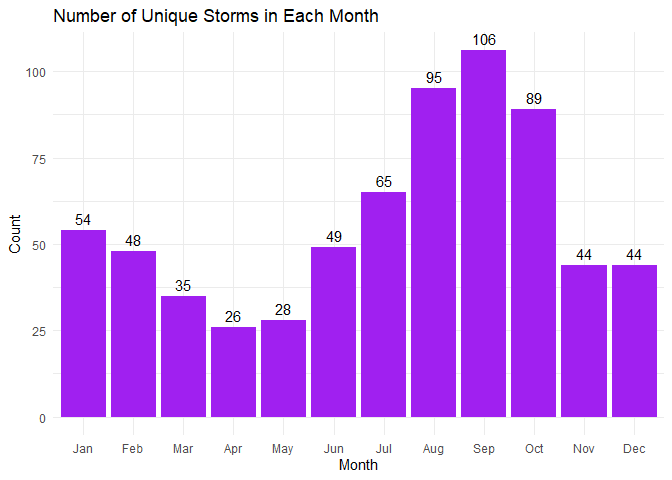
\includegraphics{workout1-elias-ghantous_files/figure-latex/unnamed-chunk-5-1.pdf}

\begin{Shaded}
\begin{Highlighting}[]
\NormalTok{storms_per_basin <-}\StringTok{ }\KeywordTok{count}\NormalTok{(}\KeywordTok{distinct}\NormalTok{(dat, basin, name), basin)}
\KeywordTok{ggplot}\NormalTok{(}\DataTypeTok{data =}\NormalTok{ storms_per_basin, }\KeywordTok{aes}\NormalTok{(}\DataTypeTok{x =}\NormalTok{ basin, }\DataTypeTok{y =}\NormalTok{ n)) }\OperatorTok{+}\StringTok{ }\KeywordTok{geom_bar}\NormalTok{(}\DataTypeTok{stat =} \StringTok{'identity'}\NormalTok{, }\DataTypeTok{fill =} \StringTok{"purple"}\NormalTok{) }\OperatorTok{+}\StringTok{ }\KeywordTok{geom_text}\NormalTok{(}\KeywordTok{aes}\NormalTok{(}\DataTypeTok{label =}\NormalTok{ n), }\DataTypeTok{vjust=}\OperatorTok{-}\FloatTok{0.5}\NormalTok{) }\OperatorTok{+}
\StringTok{  }\KeywordTok{xlab}\NormalTok{(}\StringTok{"Basin"}\NormalTok{) }\OperatorTok{+}\StringTok{ }\KeywordTok{ylab}\NormalTok{(}\StringTok{"Count"}\NormalTok{) }\OperatorTok{+}\StringTok{ }\KeywordTok{ggtitle}\NormalTok{(}\StringTok{"Number of Unique Storms By Basin"}\NormalTok{) }\OperatorTok{+}\StringTok{ }\KeywordTok{theme_minimal}\NormalTok{()}
\end{Highlighting}
\end{Shaded}

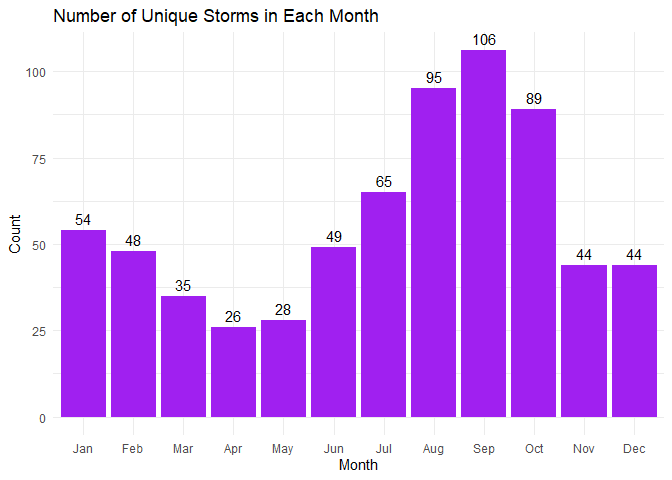
\includegraphics{workout1-elias-ghantous_files/figure-latex/unnamed-chunk-6-1.pdf}

\begin{Shaded}
\begin{Highlighting}[]
\NormalTok{stormdurations <-}\StringTok{ }\KeywordTok{count}\NormalTok{(}\KeywordTok{distinct}\NormalTok{(dat, serial_num, iso_time), serial_num)}
\NormalTok{stormdurations <-}\StringTok{ }\KeywordTok{mutate}\NormalTok{(stormdurations, }\DataTypeTok{duration_days =}\NormalTok{ (n}\OperatorTok{-}\DecValTok{1}\NormalTok{)}\OperatorTok{/}\DecValTok{4}\NormalTok{)}
\KeywordTok{summary}\NormalTok{(stormdurations}\OperatorTok{$}\NormalTok{duration_days)}
\end{Highlighting}
\end{Shaded}

\begin{verbatim}
##    Min. 1st Qu.  Median    Mean 3rd Qu.    Max. 
##   0.500   5.000   7.750   8.398  11.000  27.000
\end{verbatim}

\begin{Shaded}
\begin{Highlighting}[]
\KeywordTok{sd}\NormalTok{(stormdurations}\OperatorTok{$}\NormalTok{duration_days)}
\end{Highlighting}
\end{Shaded}

\begin{verbatim}
## [1] 4.742291
\end{verbatim}

\begin{Shaded}
\begin{Highlighting}[]
\NormalTok{max_wind_per_storm <-}\StringTok{ }\KeywordTok{as_tibble}\NormalTok{(}\KeywordTok{summarize}\NormalTok{(}\KeywordTok{group_by}\NormalTok{(dat, name, season), }\DataTypeTok{max_wind =} \KeywordTok{max}\NormalTok{(wind)))}
\NormalTok{max_wind_per_storm <-}\StringTok{ }\KeywordTok{arrange}\NormalTok{(max_wind_per_storm, }\KeywordTok{desc}\NormalTok{(max_wind))}
\KeywordTok{slice}\NormalTok{(max_wind_per_storm, }\DecValTok{1}\OperatorTok{:}\DecValTok{10}\NormalTok{)}
\end{Highlighting}
\end{Shaded}

\begin{verbatim}
## # A tibble: 10 x 3
##    name     season max_wind
##    <chr>     <int>    <dbl>
##  1 PATRICIA   2015      185
##  2 CELIA      2010      140
##  3 MARIE      2014      140
##  4 AMANDA     2014      135
##  5 DORA       2011      135
##  6 IGOR       2010      135
##  7 JIMENA     2015      135
##  8 JOAQUIN    2015      135
##  9 CRISTINA   2014      130
## 10 OLAF       2015      130
\end{verbatim}


\end{document}
